\addchap{auditorium}

\begin{wrapfigure}{l}{3.7cm}

\includegraphics[width=.95\linewidth]{img/auditorium_logo}
\end{wrapfigure}

Wenn du im Internet suchst, findest du nur unübersichtliche Foren?
Wikipedia kann dir auch nicht weiterhelfen?
Deinem Dozenten oder Tutor willst du keine E-Mail schreiben, weil du denkst, dass deine Frage unangebracht ist?

Keine Panik!
Wir haben die Lösung: auditorium.

Mit auditorium bieten wir dir die Möglichkeit, dass du zu den einzelnen Lehrveranstaltungen Fragen stellen kannst.
Diese können von deinen Kommilitonen oder den Lehrenden beantwortet, kommentiert und bewertet werden.
Wurde eine Antwort, ein Kommentar oder eine Bewertung zu deiner Frage abgegeben, wirst du darüber informiert und kannst direkt nachschauen.

Um immer die wichtigsten Fragen und Neuigkeiten zu erfahren, bietet auditorium die Möglichkeit, Lehrveranstaltungen zu verfolgen.
Folgst du einer Lehrveranstaltung, so bekommst du bei wichtigen Informationen, neuen Fragen oder Antworten eine Nachricht und weißt, was gerade wichtig ist.

{
\centering
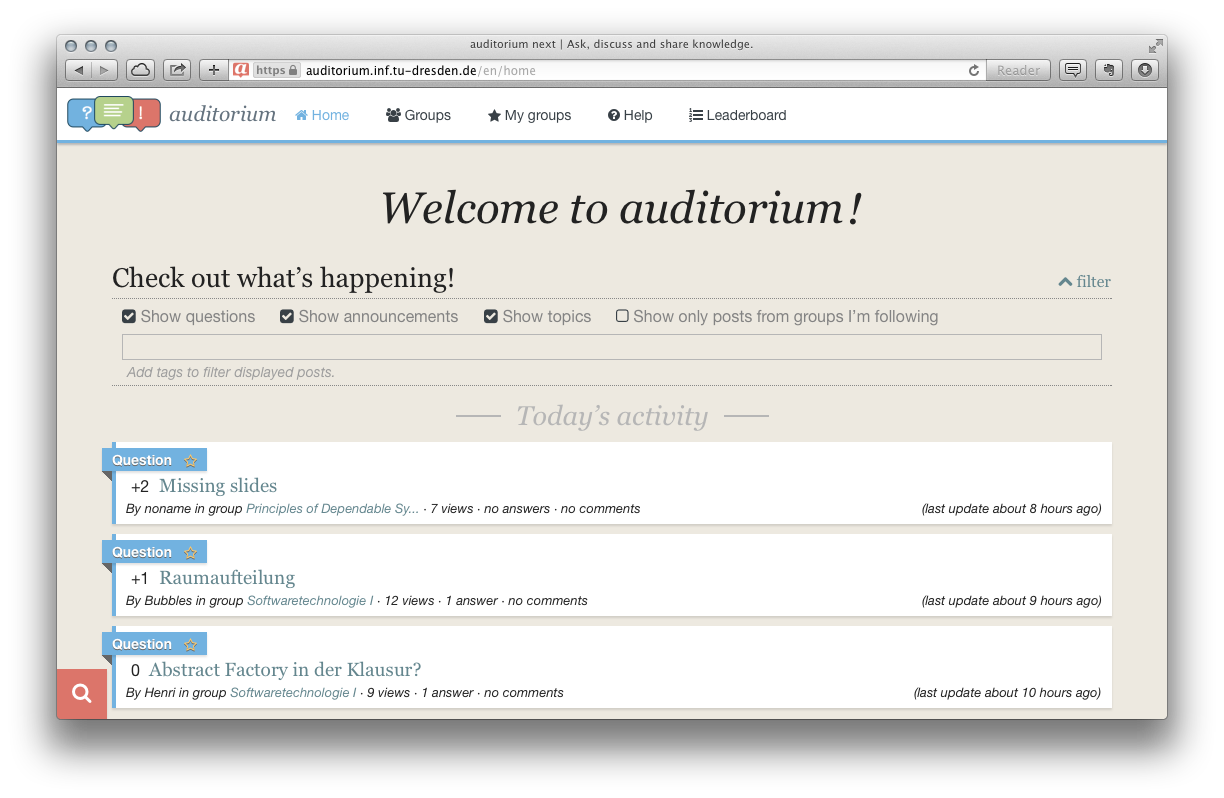
\includegraphics[width=.75\linewidth]{img/auditorium.png}
\par
}

Aber als ob das nicht schon hilfreich wäre, entwickeln wir auditorium stets weiter.
Wir haben uns dazu entschlossen, den Quellcode auf GitHub \link{https://github.com/auditorium/auditorium} zur freien Verfügung zu stellen.
Dort kann ihn jeder herunterladen und an der Entwicklung teilnehmen.
Falls du dazu Fragen oder Interesse hast, dann folge uns entweder auf Twitter \textit{@\_auditorium} oder schreibe uns eine Mail an \textit{inf-auditorium@groups.tu-dresden.de}.
